%% This is an example first chapter.  You should put chapter/appendix that you
%% write into a separate file, and add a line \include{yourfilename} to
%% main.tex, where `yourfilename.tex' is the name of the chapter/appendix file.
%% You can process specific files by typing their names in at the 
%% \files=
%% prompt when you run the file main.tex through LaTeX.

\chapter{Introduction}

The cost effectiveness and reachability of COTS elements, shrinking size of electronics serve as a perfect environment for small flying vehicles to emerge. 
This accelerating trend towards small but capable flying vehicles is pushing the limits of both hardware and software potentials of industry and academia. 
Increasing usage of these vehicles for a variety of missions pushes a further liability to secure the flight. With the advent of the new era of UAS, different institutions all over the world, specifically National Aeronautics and Space Administration (NASA) 
\cite{kopardekarunmanned} and Federal Aviation Administration (FAA) \cite{FAA_UASintegration} in US, European Aviation Safety Agency (EASA) \cite{A_NPA_EASA2015} in Europe and international bases such as International Civil Aviation Organization (ICAO) \cite{ICAO_Circular} are addressing safe integration of UAS in airspace \cite{baskaya2016flexible}.

\section{Motivation}

Improvement of the reliability of the flight is considered to be one of the main goals for integrating UAVs into civil airspace according to Unmanned systems roadmap by US Office of the Secretary of Defense, DoD \cite{UnmannedSystemsRoadmapDoD}. 
To achieve a safe flight is not an easy task considering the unknowns of the systems hardware, environment and possible system faults and failures to emerge. 
Also, increasing demand on cost effective systems, resulting in the smaller sensors and actuators with less accuracy, impose the software to achieve even more. 
The expectation that UAVs should be less expensive than their manned counterparts might have a hit on reliability of the system. Cost saving measures other than the need to support a pilot/crew onboard or decrement in size would probably lead to decrease in system reliability.

Under the research and development programs and initiatives identified by DoD in order to develop technologies and capabilities for UAS, the biggest chunk in control technologies is the health management and adaptive control with a budget of 74.3 M dollars. 
Other safety features such as validation and verification of flight critical intelligent software is the second with 57.8 M dollars \cite{UnmannedSystemsRoadmapDoD}. 

With the last turn in popularity and practicality contest among research topics of the last decade, machine learning and drones seem to be neck to neck. The sides of the race are mostly supported by high tech rather than the public who has concerns in both opponents. Is there a chance that these two can run side by side with cheers? Machine learning guides various aspects of our lives even without noticing it due to its abrupt introduction via the bigger tech companies. Its abilities rise, defeating 9-dan Go professional, their accuracy increase, enabling smooth voice recognition, adding intelligence to our daily lives. Another machine, who wants to enjoy this enabling technology is a drone. Drones, although still very strictly regulated in most countries have been spreading with great passion along their enthusiasts. Machine learning has already started to take part in aviation.

Systems are often susceptible to faults of different nature. Existing irregularities in 
sensors, actuators, or controller Fig.~\ref{fig:faultsInTheSystem} could be amplified due to the control system design 
and lead to failures. A fault could be hidden thanks to the control action \cite{ducard2009fault}.

\begin{figure}
\begin{center}
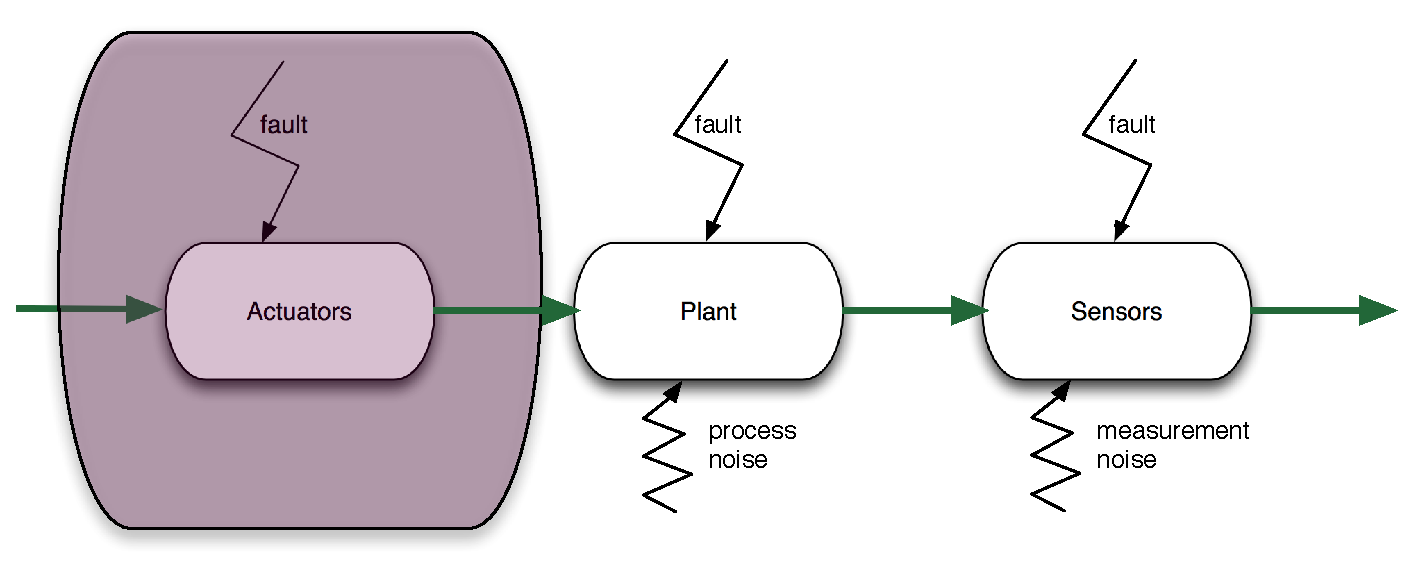
\includegraphics[width=15cm]{figures/faultsInTheSystem}    % The printed column width is 8.4 cm.
\caption{Faults altering the system } 
\label{fig:faultsInTheSystem}
\end{center}
\end{figure}




\section{Terminology}\label{ch1:opts}

Since fault tolerant control is comprised of a set of different disciplines and a relatively 
new topic, the terminology is not solid. FDI could be a proper example to this ambiguity. 
In some works, it stands for Fault Detection and Isolation while in some other 
Fault Detection and Identification, which could also named after Fault Detection and Diagnosis, 
meaning that identification is added to Fault Detection and Isolation \cite{zhang2008bibliographical}.

One of the first attempts to unify the terminology is carried out by IFAC SAFEPROCESS 
technical committee in 1996 and published by \cite{isermann1997trends}. Fault, failure, 
and the methodology to handle those such as fault detection, fault isolation, fault identification, 
fault diagnosis and supervision terms explained separately to avoid the ongoing ambiguity 
in this field. Although fault detection methods are clearer in the work, difference between 
the methods for two steps of fault diagnosis, namely the fault isolation and fault 
identification is not very obvious

\section{Conventions for a Safe Flight}\label{ch1:conventions}

The widely used method to increase reliability is to use more reliable components 
and/or hardware redundancy. Both requires an increase in the cost of the UAS 
conflicting one of the main reasons of UAS design itself band consumer expectations 
\cite{angelov2012sense}. To offer solutions for all different foreseen categories of 
airspace, a variety of approaches should be considered. While hardware redundancy 
could cope with the failure situations of UAVs in the certified airspace, it may not be 
suitable for UAVs in open or some subsets of specific categories due to budget 
constraints. Analytical redundancy is another solution, may be not as effective and 
simple as hardware redundancy, but relies on the design of intelligent methods to 
utilize every bit of information onboard aircraft wisely to deal with the instances.  

There are three approaches to achieve safe FTC in standard flight conventions. 
First one is the fail operational systems which are made insensitive to any single 
point component failure. The second approach is the fail safe systems where a 
controlled shut down to a safe state is practiced whenever a critical fault is pointed 
out by a sensor. The level of degradation assures to switch to robust (alternate) or 
direct (minimal level of stability augmentation independent of the nature of the fault) mode. 
Switching from nominal mode to the robust and direct modes leads to a decrease 
in the available GNC functions. This causes a degradation in ease of piloting. And 
also some optimality conditions could have been compromised. The third approach 
is fault tolerant control systems in which redundancy in the plant and the automation 
system is employed to design software that monitors the components and takes in 
action whenever needed. The strategy is most probably to try to keep plant availability 
and accept reduced performance \cite{blanke2000fault}.

RECONFIGURE project of FP7 \cite{goupil2015overview} aims to attack at this 
problem of piloting degradation and optimality compromisation by attacking 
Flight Parameter Estimation (FPE) which is the online estimation of aircraft parameters, 
FDD and FTC in case of off-nominal events \cite{RECONFIGURE} They utilize a black 
box nonlinear model of aircraft and The project uses some outputs of a previous FP 7 
project ADDSAFE leaded by Deimos Space \cite{ADDSAFE}.

\section{Methods for Fault Tolerant Control Systems}\label{ch1:methodsFTCS}

Among different categorizations for the fault tolerance, there are options to handle 
faults on-line or off-line. Employing fault diagnosis schemes on-line is a way to 
achieve fault tolerance. In this case, as soon as a fault detected, a supervisory 
agent is informed via a discrete event signal. Then accommodation of the faults 
are handled either with the selection of a predetermined controller for the specific 
fault case, or by designing the action online with real-time analysis and optimization \cite{blanke2000fault}.

Another common categorization of FTCS is passive and active FTCS. In passive FTCS, 
the flight controller is designed in such a way to accommodate not only the 
disturbances but also the faults. Active FTCS first distinguishes the fault via fault detection 
and diagnosis module and then switch between the designed controllers specific to the 
fault case or design a new one online \cite{angelov2012sense}. While active FTCS 
requires more tools to handle faults as seen in Fig.~\ref{fig:FTCS}, for faults 
not predicted and not counted for during the design of the robust controller, this method 
most probably fails. 

\begin{figure}
\begin{center}
%\includegraphics[width=11.3cm]{figures/FTCmethods}    % The printed column width is 8.4 cm.
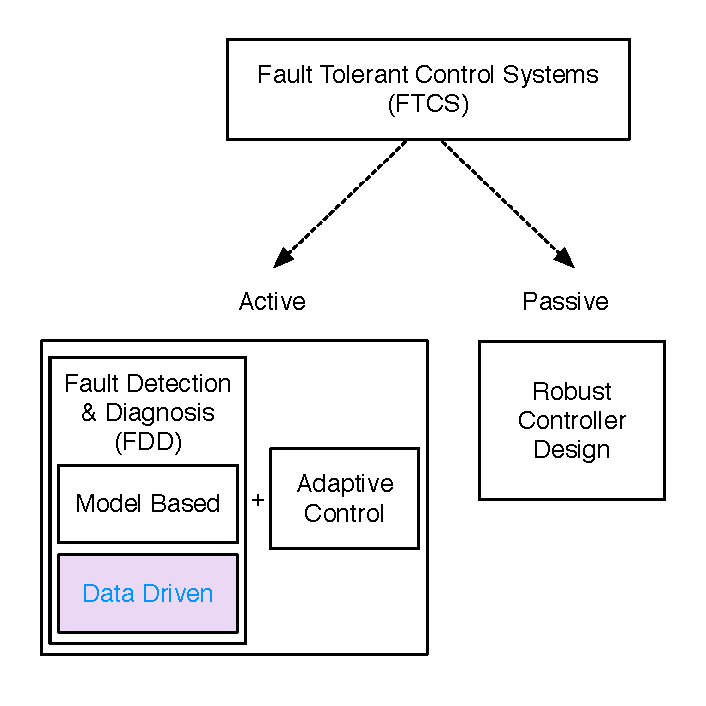
\includegraphics[width=11.3cm]{figures/FTCS}
\caption{Variations of fault tolerant control systems } 
\label{fig:FTCS}
\end{center}
\end{figure}


Even with a long list of available methods, aerospace industry has not implemented 
FTC widely, except some space systems, due to the evolving nature of the methods, 
the tricks coming with the nonlinear nature of the problem, design complexity and high 
possibility of wrong alarms in case of large disturbances and/or modeling uncertainties. 
So the already carried reliability measures concerning the hardware redundancy is 
now the preferred way because of its ease and maturity being implemented on various 
critical missions with considering human lives.

\subsection{Fault Detection and Diagnosis}

FDD is handled in two main steps; fault detection and fault diagnosis. Fault diagnosis 
encapsulates fault isolation and fault identification. The methods for detection and 
diagnosis are investigated for their frequency of utilization separately for sensor, 
actuator, process and controller faults in \cite{isermann1997trends}. FDD should 
not only be sensitive to the faults but also robust to the model uncertainties and 
external disturbances.

Two distinct options to proceed in analytical redundancy are the model based 
approaches and data-driven approaches. They form the two ends of a continuous 
solution set line, so utilizing them in a combination might end up with better solutions. 
Model based fault diagnosis highlights the components of a system and the connections 
in-between, and their corresponding fault modes. Data driven fault diagnosis rely on 
the observational data and prefers dense, redundant and with a  frequency larger than 
the failure rate. 

% This is an example of how you would use tgrind to include an example
% of source code; it is commented out in this template since the code
% example file does not exist.  To use it, you need to remove the '%' on the
% beginning of the line, and insert your own information in the call.
%
%\tagrind[htbp]{code/pmn.s.tex}{Post Multiply Normalization}{opt:pmn}

\subsubsection{Model Based Methods}

In model based approaches, relations between measurements and estimated 
states are exploited to detect possible dysfunction. The most common ways to 
implement a model based approach is to estimate the states, estimate the model 
parameters, or parity-space. The accuracy of the results depend on the type of 
faults (additive or multiplicative). Additive faults affects the variables of the process 
by a summation whereas the multiplicative faults by a multiplication.  When only 
output signal can be measured, signal model based methods can be employed for 
fault detection such as Bandpass filters, Spectral analysis(FFT) and maximum entropy estimation. 
For the case, both the input and output signals are available, the utilized methods 
for fault detection are called the process based methods: State and output 
observers(estimators), Parity equations and Identification and parameter estimation. 
They generate residuals for state variables or output variables. When previous works 
investigated, it is concluded that the most widely used technique for sensor and actuator 
faults is the state and output observers (estimators) and for process faults, identification 
and parameter estimation \cite{isermann1997trends}.

The output of the model based fault detection methods is the stochastic behaviour 
with mean values and variances. With the use of change detection methods, deviations 
from the normal behavior can be detected. For that purpose, three available methods 
considered are, mean and variance estimation, likelihood-ratio-test and Bayes decision, 
run-sum test andtwo-probe t-test. Fault detection is only supported by simple threshold 
logic or hypothesis testing in most of the applications \cite{isermann1997trends}.

A bunch of studies discovers the band of different approaches for model-based fault detection. 
Detecting sensor and actuator faults via state estimation, utilizing an EKF is applied to a 
F-16 model in \cite{hajiyev2005sensor}. Parameter identification via $H_{\infty}$ filter 
is used to indicate icing in \cite{melody2001h}.

A drawback of model-based approaches is that they require accurate model of the 
aircraft for successful detection. In a small UAV system susceptible to various 
uncertainties/disturbances and most of the cases does not have an accurate model, 
leading a model-based approach might fail. And also, a mathematical model of a UAV 
is constructed within the flight envelope, and does not necessarily describe the 
possible dynamics invoked by a failure on-board.

A way to handle that is to offer solutions to cope with the uncertainties. 
A fairly old study in 1984, investigates the design problem FDI systems robust to 
uncertainties within the models. One of the two steps of FDI, two steps being the 
residual generation and decision-making, is targeted. They offer to handle model 
uncertainties, by designing a robust residual generation process \cite{chow1984analytical}. 
Another study deals with model uncertainties by determining the threshold of the residual 
in a novel way with an application to detect aileron actuator fault \cite{rotstein2006fault}. 
\cite{sharma2007fault} utilize two cascade sliding mode observers state estimation and 
fault detection to guarantee staying in sliding manifold in the presence of unknown 
disturbances and faults. 
% This is an example of how you would use tgrind to include an example
% of source code; it is commented out in this template since the code
% example file does not exist.  To use it, you need to remove the '%' on the
% beginning of the line, and insert your own information in the call.
%
%\tgrind[htbp]{code/be.s.tex}{Block Exponent}{opt:be}

\subsubsection{Data-Driven Methods}

Model-based approaches had various successful applications until now, 
most of them assuming accurate model is available on-board. With the new 
era of UAVs, the airspace is expected to be populated by an abrupt increase 
in the number of UAVs. The variety of UAVs, expense of accurate modeling 
practices, the difficulty in modeling the behavior of UAV in case of failures, 
call for alternative approaches for the quite challenging problem of FDD. 
The increased efficiency of sensors on-board, the increase in the computational 
capabilities of autopilot processors, and the advances in machine learning 
techniques in the last decade may offer efficient data-driven solutions to FDD.

In data driven methods, a detailed knowledge about the internal dynamics 
of the system is not necessary. The data available is the source of information 
with regard to the behavior of the system. Supervised learning, which requires 
to label the fault cases previously in the training data, is usually utilized for 
data-centric inference of causes. In case of an unlabeled fault, the result is 
expected as a probability distribution of the available normal modes, identified 
fault labels and a probable unknown fault. What is needed at that point is to 
first detect and localize the fault and then to consult domain experts for labeling 
for further integration of this fault into the diagnosis scheme \cite{dataCentricDiagOffline}.

\cite{gui2002fault} argues artificial intelligent methods for fault detection of complex 
systems. Comparison between PCA and model based stochastic parity space 
approaches is given in \cite{hagenblad2004comparison}.
In \cite{li2016data}, the authors argues to use dynamic PCA since UAV flight 
controls is a dynamic system itself and DPCA can reflect unknown disturbances, 
while model-based approaches can only model typical disturbance.  